

As metodologias de software proporcionam um conjunto de práticas e plano de trabalho que se alinha com as demandas do projeto permitindo que impulsionem a produtividade e proporcione o desenvolvimento de um produto de maior valor \cite{kent_2004}. Sendo assim, a metodologia de desenvolvimento deste trabalho segue princípios de práticas ágeis e une características do Extreme Programming (XP) ao Scrum, Kanban e Lean Inception. 

No que diz respeito a metodologias ágeis, os atributos de programação em pares, aplicação de testes automatizados com TDD e a refatoração foram aproveitados da metodologia XP \cite{highsmith_2000}. Já as características extraídas da metodologia Scrum foram os conceitos de sprints iterativas e incrementais, junto das reuniões diárias \cite{schwaber_scrum_2013}. Vale destacar que esta última metodologia coube adaptações no contexto de uma equipe reduzida. 

O Kanban, por sua vez, foi adotado como uma ferramenta de gestão visual para acompanhar o andamento das tarefas. Por fim, o Lean Inception estruturou a definição e priorização do Mínimo Produto Viável (MVP), que possibilitou a conformidade entre os envolvidos sobre a ideia do produto final.

%--------------------------------------------------------------------------


\subsection{Metodologia Ágil}


As metodologias ágeis foram criadas no final dos anos 1990 e seu principal objetivo era solucionar as limitações dos métodos tradicionais de desenvolvimento de software, que frequentemente resultavam em produtos inflexíveis e com longos ciclos de entrega \cite{kent_2004}.

Dessa forma, o projeto proposto busca adotar metodologias ágeis como maneira de garantir maior flexibilidade, caso seja necessário a realização de ajustes, e proporcionar um processo mais produtivo, além de mitigar riscos ao longo do ciclo de vida do software.


%--------------------------------------------------------------------------


\subsection{Extreme Programming (XP)}

O objetivo do Extreme Programming é o desenvolvimento de um software robusto. Com o uso dessa metodologia de desenvolvimento, é possível desenvolver softwares com menos defeitos, com menor custo e com maior produtividade \cite{kent_2004}. Sendo assim, a utilidade dessa metodologia é justificada pela ênfase na qualidade do código e eficiência das práticas de programação.

O XP segue quatro valores fundamentais: a \textbf{comunicação}, onde o time deve ser capaz de expressar suas opiniões e se comunicar de maneira eficaz; \textbf{simplicidade}, priorizando soluções simples para atingir objetivos propostos; \textbf{coragem}, onde o desenvolvedor deve ter a disposição para refatorar e implementar sem receio; por fim, \textbf{feedback}, a fim de receber retorno construtivo \cite{kent_2004}. Sendo assim, a junção desses valores favorece o desenvolvimento eficaz, abrindo espaço para inovação e novas soluções.

Segundo \citeonline{highsmith_2000}, o  Extreme Programming possui 12 práticas desejaveis, sendo elas:

\begin{enumerate}
    \item Planejamento;
    \item Entregas frequentes;
    \item Metáfora;
    \item Projeto simples; 
    \item Testes;
    \item Refatoração;
    \item Programação em pares; 
    \item Propriedade coletiva; 
    \item Integração contínua; 
    \item 40 horas semanais; 
    \item Cliente presente; 
    \item Código padrão.
\end{enumerate}

Entretanto, devido ao escopo do projeto, não é viável adotar todas as 12 práticas. As práticas consideradas mais adequadas para este projeto são: programação em pares, testes, com ênfase em TDD e refatoração.

\subsubsection{Test-Driven Development (TDD)}

Com o intuito de promover o desenvolvimento e melhorar a qualidade do código, é utilizado o Test-Driven Development (TDD). Essa abordagem consiste em escrever testes automatizados antes de implementar novas funcionalidades. O ciclo segue o seguinte fluxo: primeiramente, se escreve um teste que irá falhar, em seguida é implementado o código para satisfazer o teste e depois a refatoração, conforme a Figura~\ref{ttdcicle}. Essa abordagem garante que o código satisfaça todos os requisitos desde o início \cite{aniche_2014}.

\begin{figure}[H]
    \centering
    \caption{Ciclo do Test-Driven Development.}
    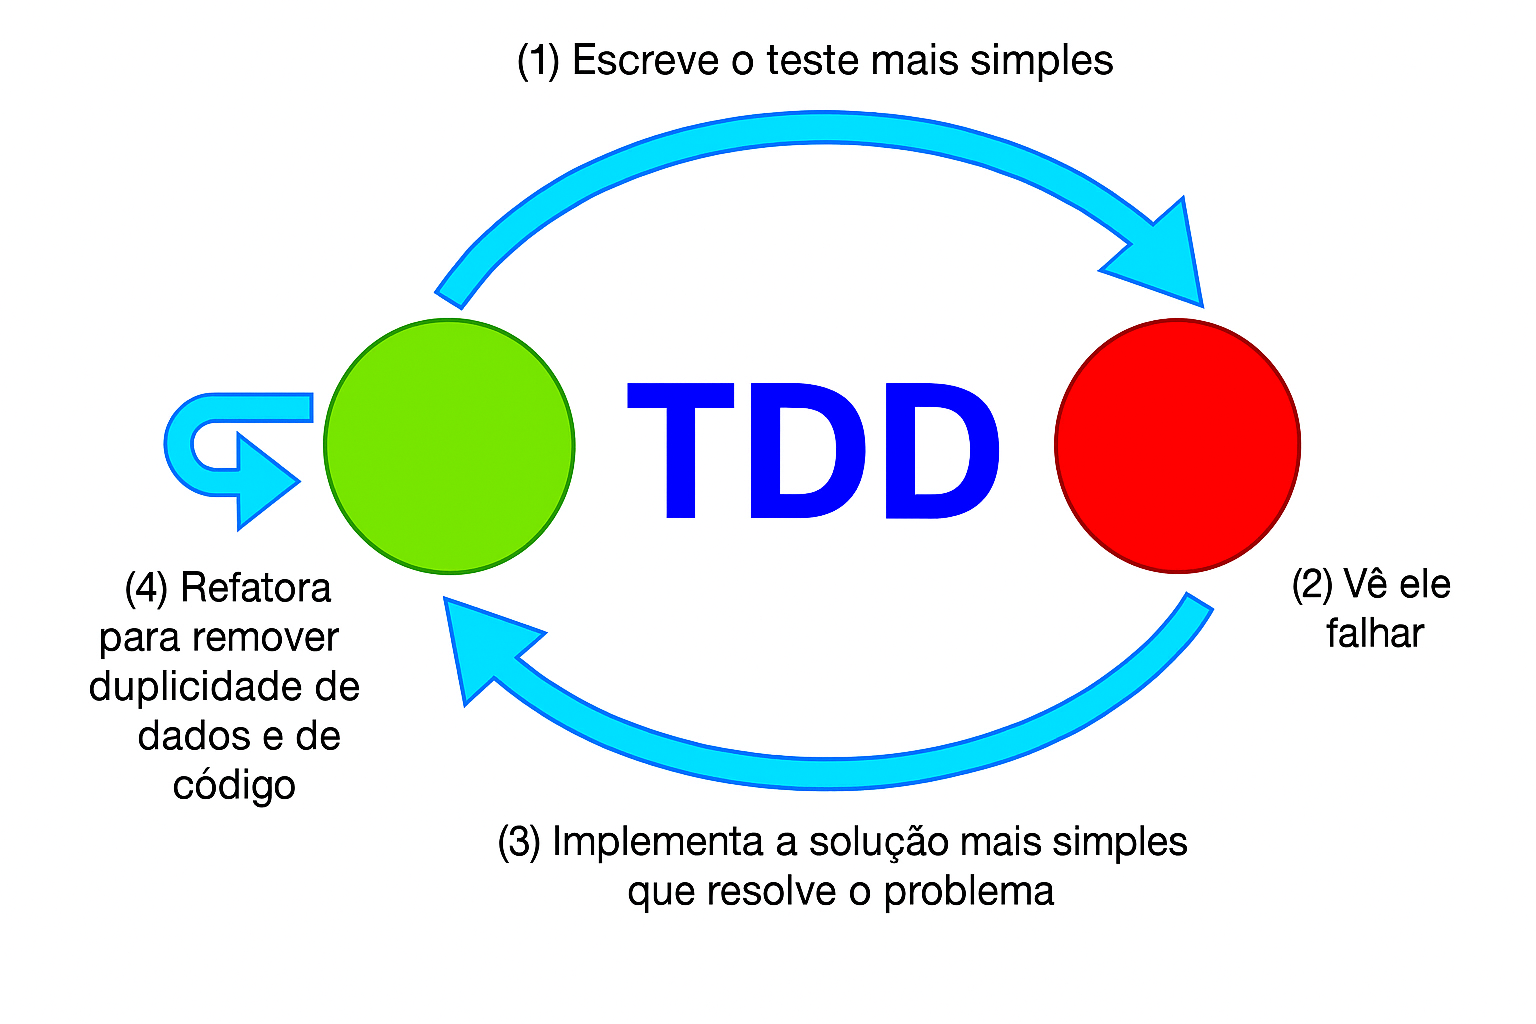
\includegraphics[width=0.8\textwidth]{figuras/ciclotdd.png}
    \par
    Fonte: \citeonline{aniche_2014}.
    \par
    \label{ttdcicle}
\end{figure}

Sendo assim, \citeonline{janzen_2005}, mostou que programadores que utilizam TDD poduzem código que passam em aproximadamente mais de 50\% dos testes caixa-preta, ademais, \citeonline{Maximilien_2003} descreveram redução em mais de 40\% de quantidade de defeitos. Além disso, ambos destacam o aumento da produtividade, devido a menor tempo debugando.

Entretanto, o TDD exige um esforço inical no ínicio do desenvolvimento, segundo \citeonline{nagappan_2006}, ocorre um aumento entre 15\% a 30\% de desenvolvimento na fase inicial, porém devido aos beneficios a longo prazo desse estilo de programação isso é aceitavel, portanto, a utilização dele se prova extremamente benéfica.


%--------------------------------------------------------------------------


\subsection{Scrum}

De certo, um dos principais \textit{frameworks} para organização e desenvolvimento é o Scrum, o mesmo é utilizado por equipes que usam \textit{sprints} iterativas a fim de enfrentar projetos de forma incremental, ou seja, a fim de solucionar um problema geral, o Scrum divide partes desse problema em \textit{sprints}, com esse processo, é gerado o artefato "Sprint Backlog" \cite{schwaber_scrum_2013}. Sendo assim, a Figura~\ref{bpmnsprint} apresenta a esquematização das \textit{sprints} utilizada neste projeto.

\begin{figure}[H]
    \centering
    \caption{BPMN Sprint.}
    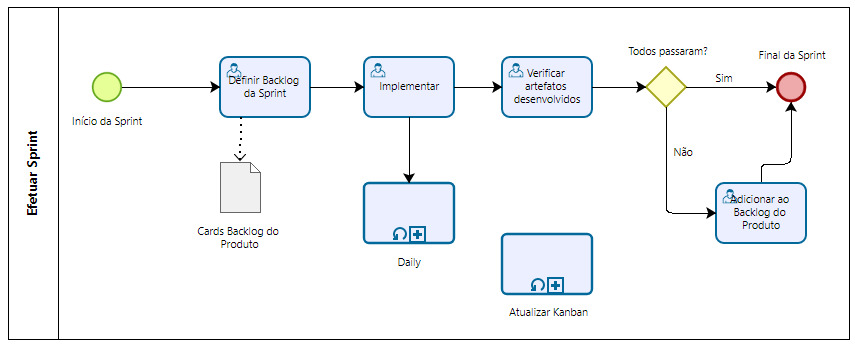
\includegraphics[width=1\textwidth]{figuras/sprint.jpeg}
    \par
    Fonte: autoria própria.
    \par
    \label{bpmnsprint}
\end{figure}

Além disso, o Scrum se baseia em três importantes pilares, sendo eles a transparência, adaptação e inspeção. A transparência é o fator que garante que os integrantes do time saibam o que está sendo feito, para isso, durante as \textit{sprints}, é realizado um processo chamado \textit{daily}, conforme visualizado na Figura~\ref{bpmndaily}, no qual os membros compartilham seus progressos, impedimentos e planos \cite{schwaber_scrum_2013}.

\begin{figure}[H]
    \centering
    \caption{BPMN Daily.}
    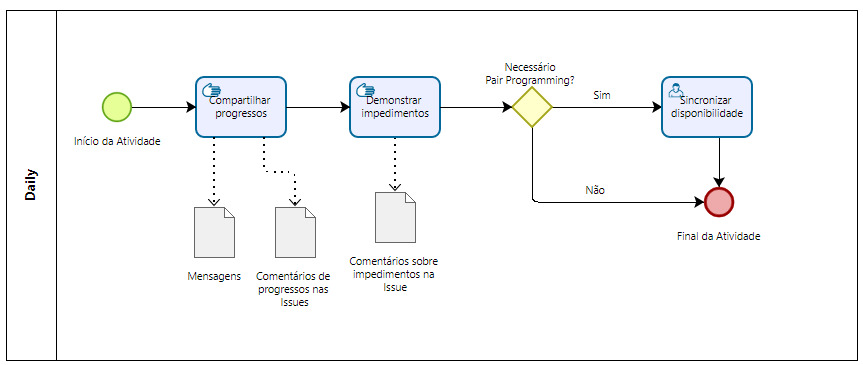
\includegraphics[width=1\textwidth]{figuras/daily.jpeg}
    \par
    Fonte: autoria própria.
    \par
    \label{bpmndaily}
\end{figure}

A adaptação é outro fator fundamental para o Scrum, o mesmo pode ser adaptado em diversos cenários, idealmente a metodologia Scrum é realizada em um time com 3 a 10 pessoas. Entretanto, devido ao grande número de empresas com somente um único desenvolvedor, foi criado o Scrum Solo, uma adaptação do Scrum e do Personal Software Process, com o objetivo de obter os benefícios do Scrum para equipes com uma única pessoa \cite{pagotto_2016}. 

Sendo assim, é possível adaptar elementos do Scrum para desenvolvimento em dupla, se baseando no conceito de Scrum Solo. O mínimo de membros para o Scrum se deve aos três principais papéis que o mesmo possui: o \textit{product owner}, \textit{scrum master} e \textit{dev team}. Logo, a fim de ocupar todos os papéis, é necessário que ambos da dupla ocupem a posição de \textit{dev team} e outra arbitrária \cite{schwaber_scrum_2013}.


%--------------------------------------------------------------------------


\subsection{Kanban}

A fim de favorecer a inspeção, um dos pilares do Scrum, é recomendado o uso do Kanban, devido à sua capacidade de fornecer uma visão clara sobre as tarefas em andamento. O Kanban é um sistema de gestão visual que utiliza cartões para exibir a situação geral das tarefas. Ainda mais, o Kanban melhora o desempenho em 50% de tarefas devido à sua capacidade de indicar e limitar o fluxo de trabalho em andamento \cite{skarin2015}.

Sendo assim, é possível definir o Kanban em três tipos principais: produção, movimentação e E-Kanban. O Kanban de Produção, que possui o intuito central de mostrar o quadro de desenvolvimento de um projeto em três baias: \textit{todo}, \textit{doing} e \textit{done}, que representam as tarefas a fazer, em desenvolvimento e feitas respectivamente, cuja lógica pode ser visualizada na figura~\ref{bpmnkanban}.

\begin{figure}[H]
    \centering
    \caption{BPMN Kanban.}
    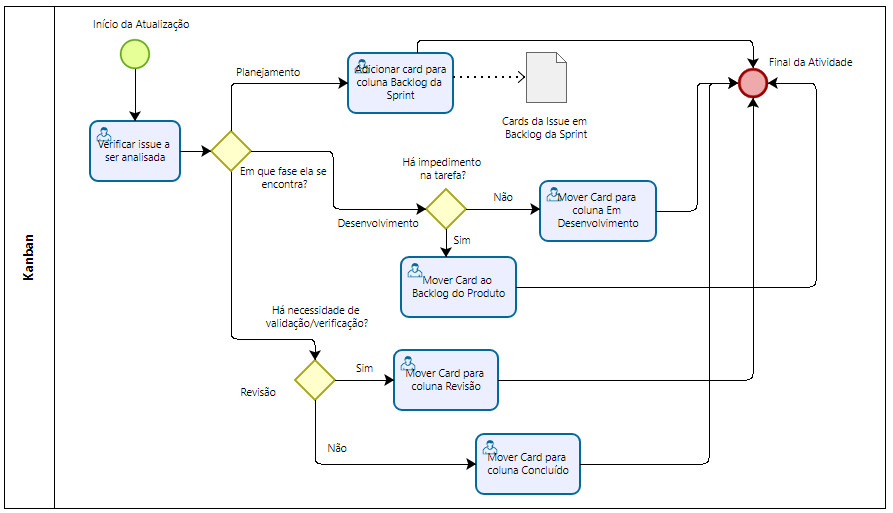
\includegraphics[width=1\textwidth]{figuras/kanban.jpeg}
    \par
    Fonte: autoria própria.
    \par
    \label{bpmnkanban}
\end{figure}

Ademais, existe o Kanban de Movimentação para gerenciar processos em produção e, por fim, o E-Kanban, que é uma versão online do Kanban de produção, utilizando softwares para auxiliar a visualização do quadro de tarefas.

Em suma, as tarefas a serem disponibilizadas no Quadro Kanban encontram-se no Backlog do Produto, no qual estão todas as tarefas previstas para o desenvolvimento do projeto proposto. Dessa forma, o uso combinado do Kankan com ferramentas de \textit{sprints} contribuirá para a organização e acompanhamento das tarefas \cite{skarin2015}. 


%--------------------------------------------------------------------------


\subsection{Lean Inception}
\label{subsec:lean_inception}

É necessário um método para a definição do mínimo produto viável (MVP). Nesse sentido, a metodologia Lean Inception se adequa a esse propósito, tendo sido desenvolvida por Paulo Caroli em 2017, conhecido por sua grande influência nas metodologias ágeis. A metodologia é amplamente utilizada para maximizar o tempo dedicado à elicitação de requisitos, partindo do mapeamento de jornadas e personas para, em seguida, priorizar as funcionalidades essenciais e definir a versão mínima do produto \cite{caroli2017lean}.

A metodologia consiste em quatro etapas distintas, que garantem que o time terá uma visão compartilhada para o produto ao longo do processo: visão de produto, identificação de usuários e necessidades, priorização de funcionalidades e, por fim, organização das funcionalidades mínimas do produto por meio dos artefatos ``Sequenciador'' e ``Canvas MVP'' \cite{caroli2017lean}. A aplicação desta metodologia exige um ambiente colaborativo e, com esse propósito, foi utilizado um template desenvolvido na plataforma Miro por \citeonline{miro_lean}.

%Logo, com as necessidades prontas, é feita a terceira fase, na qual é realizada a priorização das funcionalidades e é desenvolvido o artefato "Revisão", onde é agregado a dificuldade de cada funcionalidade. Enfim, na última fase é feito o "Sequenciador" e "Canvas do MVP" que organizam as funcionalidades mínimas para o produto \cite{caroli2017lean}.
%
%Por fim, a aplicação desta metodologia exige um ambiente colaborativo, e, com esse propósito foi desenvolvido um template na plataforma Miro por \citeonline{miro_lean}, com o intuito de viabilizar a realização dessa dinâmica.

%MELHORAR ISSO:
Como resultado da primeira etapa, foi definida a visão geral do produto: um pwa, multiplataforma, gratuito e open source, voltado a estudantes e profissionais do meio universitário que necessitam de auxílio psicológico ou desejam adotar hábitos saudáveis. O produto, denominado Seed, tem como diferencial auxiliar os indivíduos em questões de saúde mental por meio da coleta de dados e da oferta de informações condizentes, além de fomentar a prática de hábitos saudáveis. diferentemente de aplicativos como o Daylio, que atuam apenas na adoção de hábitos saudáveis.

Ao final da metodologia, é elaborado o Canvas MVP, que consolida as principais definições do produto mínimo viável em sete blocos: proposta do MVP, personas segmentadas, jornadas, funcionalidades, resultado esperado, métricas para validar as hipóteses de negócio, e custos e cronograma \cite{caroli2017lean}. A Figura \ref{canvamvpf} apresenta o Canvas MVP elaborado para o projeto.

\begin{figure}[H]
    \centering
    \caption{Canvas MVP (Seed).}
    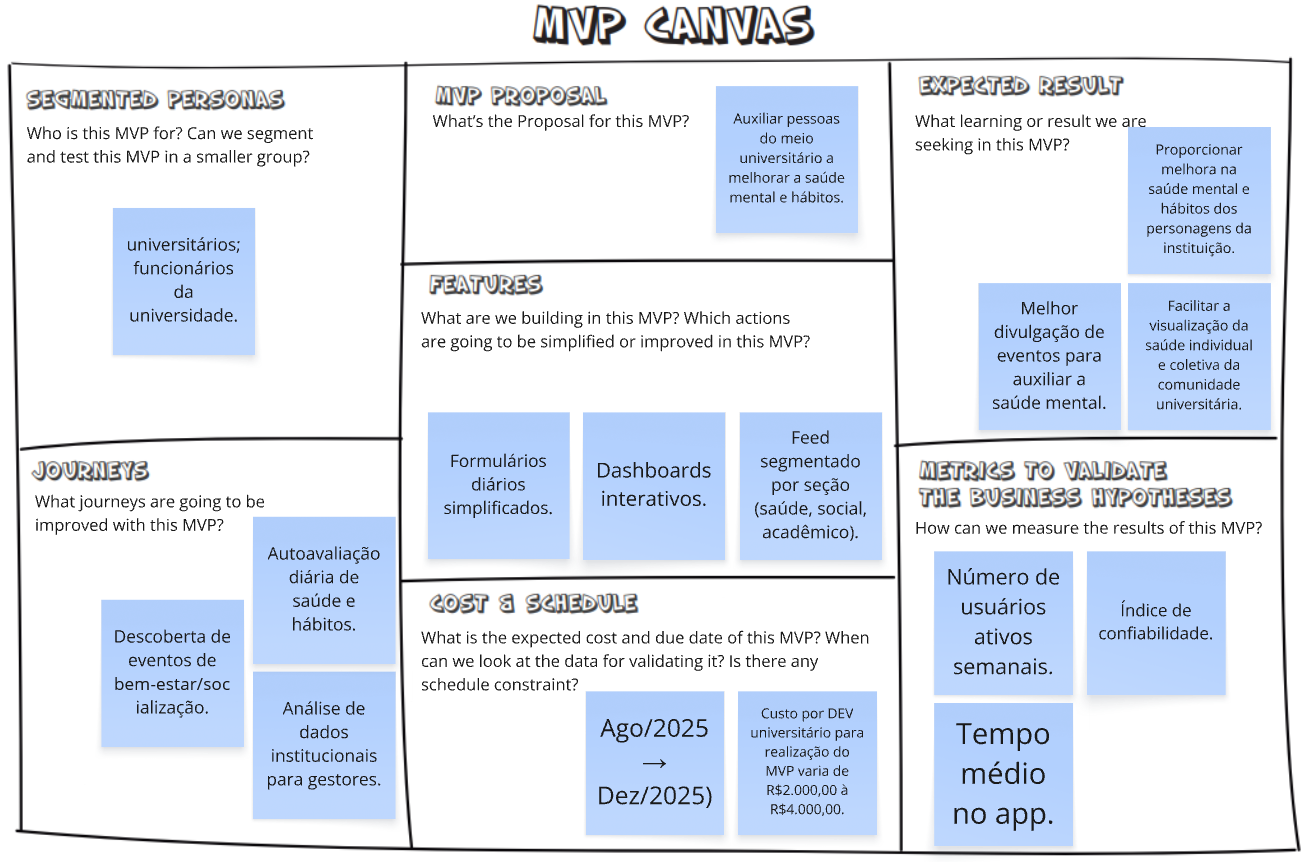
\includegraphics[width=1\textwidth]{figuras/mvpcanvas.png}
    \par
    Fonte: autoria própria com base em \citeonline{caroli2017lean}.
    \par
    \label{canvamvpf}
\end{figure}

Os demais artefatos produzidos durante a aplicação da metodologia, Visão de Produto, É - Não É - Faz - Não Faz, Objetivos do Negócio, Personas, Jornadas de Usuário, Brainstorming de Funcionalidades, Revisão e Sequenciador, encontram-se detalhados no Apêndice \ref{apendice:lean_inception}.

%--------------------------------------------------------------------------

\subsection{Questionário}

O questionário é uma ferramenta eficiente para a obtenção de dados quantitativos e qualitativos de um público-alvo extenso \cite{vazquez2016engenharia}. Com o intuito de complementar o escopo do produto a ser desenvolvido com base na perspectiva dos possíveis usuários, foi elaborado o questionário apresentado no Apêndice~\ref{apendice:questionario}.

A primeira pergunta vista na Figura ~\ref{q2} tem como objetivo filtrar o público alvo do formulário. Dessa forma as respostas coletadas das questões subsequentes restringem-se apenas à parte interessada - esta que está inserida na cenário universitário. Além disso, optou-se por colher os dados da comunidade atual a fim de analisar o perfil presente dos indivíduos inseridos no contexto universitário.

As duas seguintes perguntas, observadas nas Figuras ~\ref{q3} e ~\ref{q4}, compõem a primeira seção do formulário e estão relacionadas ao tempo de permanência na instituição e ao respectivo campus do participante do formulário aplicado. Tais informações são relevantes para a análise prévia da presença de correlações entre estes dados com as autoavaliações de determinantes da saúde do colaborador - estas representadas nas Figuras ~\ref{q5}, ~\ref{q6} e ~\ref{q7}, que constituem a segunda seção do formulário.

Assim, os determinantes da saúde relevantes e considerados acessíveis de serem tratados por projetos elaborados pela universidade foram avaliados. Ademais, foram coletados dados qualitativos a respeito da presença de demais variáveis da saúde, que identificaram outros tópicos, sendo eles: \textbf{(1) }acessibilidade na instituição; \textbf{(2)} vida financeira; \textbf{(3)} acesso a cultura e \textbf{(4)} vida amorosa. Esses resultados estão ilustrados nas Figuras ~\ref{q8} e ~\ref{qa}.

Por fim, na terceira seção do inquérito, torna-se evidente a necessidade do desenvolvimento de uma alternativa tecnológica de promoção da saúde na Universidade de Brasília (UnB). Isso porque é possível verificar na Figura ~\ref{q9} que 58\% dos participantes acreditam que sua instituição de ensino não possui serviços de apoio a saúde mental ou de fomentação de bons hábitos de vida. Tendo em vista que nesta coleta de dados, apenas um dos interrogados não está inserido na UnB, trata-se de um dado alarmante, já que esta é formalmente vista como promotora da saúde.

A justificativa do desenvolvimento deste software também se alicerça na Figura ~\ref{q10} que mostra uma aceitação de 58\% dos participantes em relação a um aplicativo voltado à saúde mental e à manutenção de hábitos de vida. Da mesma forma, os dados previamente vistos nas Figuras ~\ref{q5} e ~\ref{q7}, que exibem uma avaliação mediana na saúde geral e preocupante no estado mental dos participantes, demonstram tal necessidade. 

Isto posto, foi avaliado na Figura ~\ref{q11} as funcionalidades que esse sistema pode dispor. As sugestões exibidas na Figura ~\ref{qb} foram adaptadas ao escopo inicial estipulado com o intuito de obter êxito neste projeto e contribuir para a promoção da saúde na Universidade de Brasília.

\subsubsection{Análise de Confiabilidade}

Um aspecto fundamental da avaliação do questionário proposto é a análise de sua confiabilidade. Para isso, foi calculado o coeficiente Alfa de Cronbach, cujo resultado foi de 0.6949, com intervalo de confiança de [0.519 0.828], indicando um nível aceitável de consistência interna para a utilização dos dados coletados.

Além disso, foi realizada uma análise de correlação entre os itens do questionário, conforme apresentado na Figura~\ref{correlacao}, cujas perguntas utilizadas estão listadas a seguir:

\begin{itemize}
    \item \textbf{P1} – Há quanto tempo você faz parte da comunidade universitária?
    \item \textbf{P2} – Caso você esteja inserido na instituição da UnB, de qual campus você faz parte?
    \item \textbf{P3} – Alimentação
    \item \textbf{P4} – Hidratação
    \item \textbf{P5} – Autoconhecimento
    \item \textbf{P6} – Vida Acadêmica
    \item \textbf{P7} – Mobilidade (facilidade de logística na rotina)
    \item \textbf{P8} – Saúde Mental
    \item \textbf{P9} – Acesso à saúde
    \item \textbf{P10} – Condição de moradia
    \item \textbf{P11} – Convívio Social (amigos, família e companheiros)
    \item \textbf{P12} – Exercício físico
    \item \textbf{P13} – Realização de hobbies
    \item \textbf{P14} – Uso de Redes Sociais
    \item \textbf{P15} – Uso de substâncias (álcool, cigarro, drogas ilícitas)
    \item \textbf{P16} – Prática de algum vício
    \item \textbf{P17} – No geral, como você avalia a sua saúde? (1 estrela para péssimo até 5 estrelas para excelente)
    \item \textbf{P18} – Você acredita que a sua instituição oferece serviços de apoio à saúde mental ou de fomentação de bons hábitos de vida?
    \item \textbf{P19} – Você usaria um aplicativo da sua instituição universitária para o acompanhamento da sua saúde mental e a manutenção de hábitos de vida?
\end{itemize}

\begin{figure}[H]
    \centering
    \caption{Matriz de correlação do questionário.}
    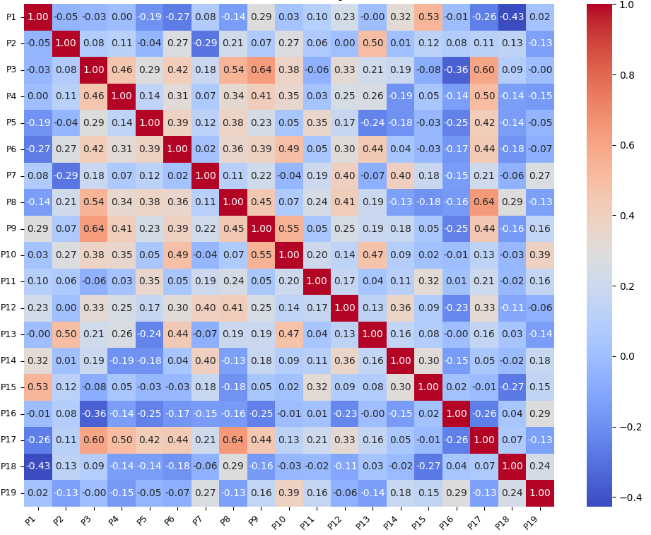
\includegraphics[width=1\textwidth]{figuras/correlacao1.png}
    \par
    Fonte: autoria própria.
    \label{correlacao}
\end{figure}

Em suma, a matriz de correlação evidencia a relação entre as variáveis, permitindo identificar possíveis padrões de associação entre os aspectos avaliados. Observa-se, por exemplo, uma correlação moderada entre os itens \textbf{P3} (Alimentação) e \textbf{P4} (Hidratação), bem como entre \textbf{P8} (Saúde Mental) e \textbf{P17} (Avaliação geral da saúde), o que sugere uma relação entre o bem-estar físico e psicológico.

Vale ressaltar, contudo, que o questionário utilizado possui natureza exploratória e estrutura simples, o que pode limitar a profundidade das análises. Ainda que os resultados indiquem padrões confiáveis dentro da amostra coletada, não se pode generalizar integralmente as conclusões para toda a população universitária.